% Funcionalidades
\section{Funcionalidades}
	\subsection{¿Que teníamos?} %ptos fuertes, ptos flacos
	\begin{frame}
		\frametitle{Una web estática}
		\begin{columns}
		\column{9cm}
			\setbeamercovered{invisible}
			\begin{itemize}
				\item <1-| alert@1> Una web estática
				\item <2-| alert@2> Difícil de mantener
				\item <3-| alert@3> Sin grandes atractivos para el usuario
				\item <4-| alert@4> Sin interactividad con el usuario
				\item <5-| alert@5> No es 2.0
				\item <6-| alert@6> Totalmente funcional
				\item <7-| alert@7> Folletos divulgativos
				\item <8-| alert@8> Un CD con el contenido de la web
			\end{itemize}

		\column{2cm}
			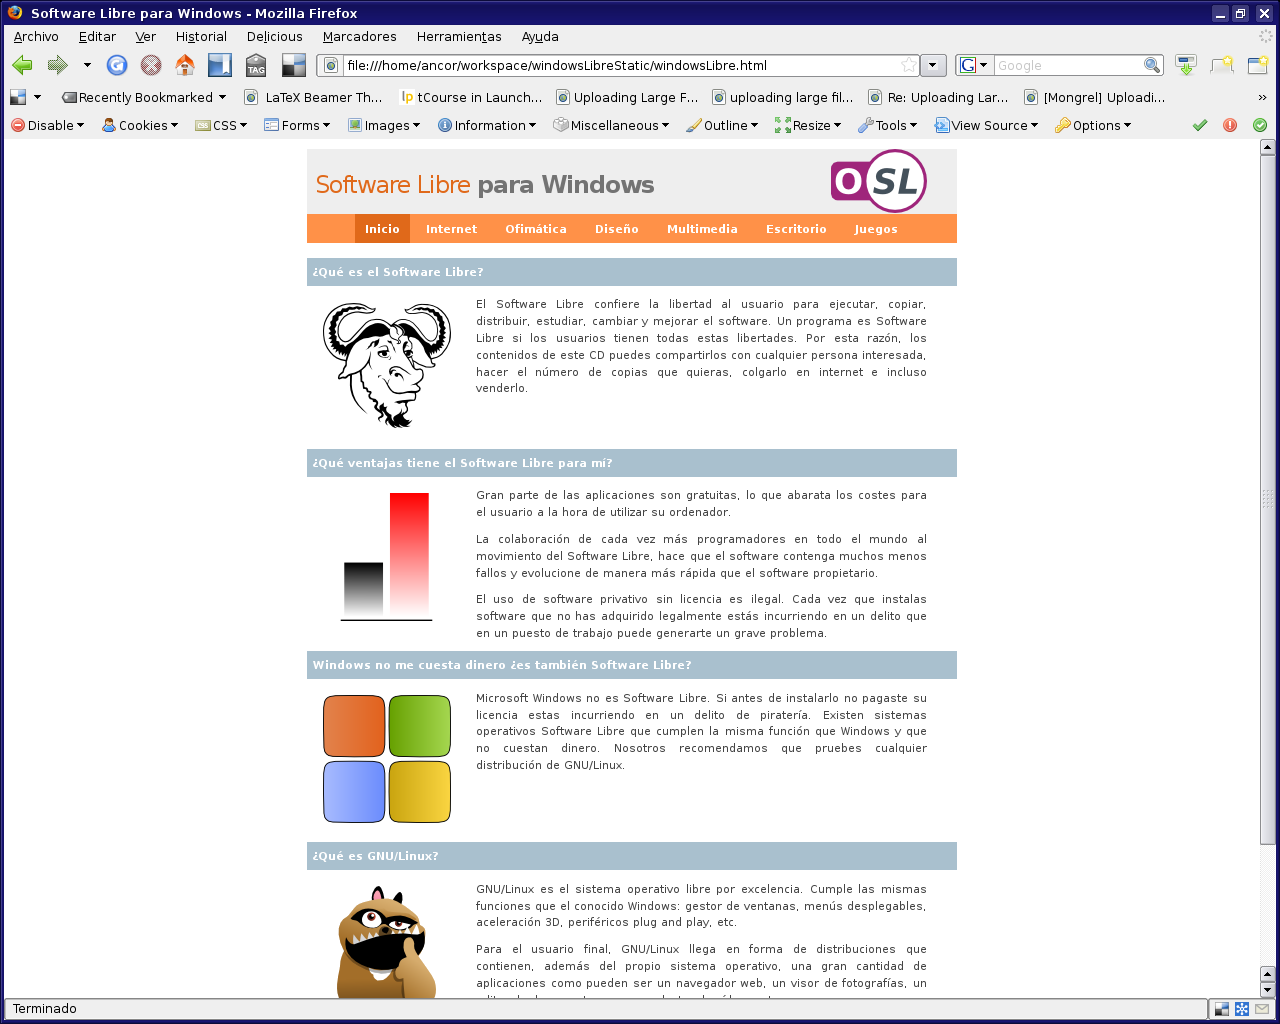
\includegraphics[width=2cm]{images/wl_old01.png}
			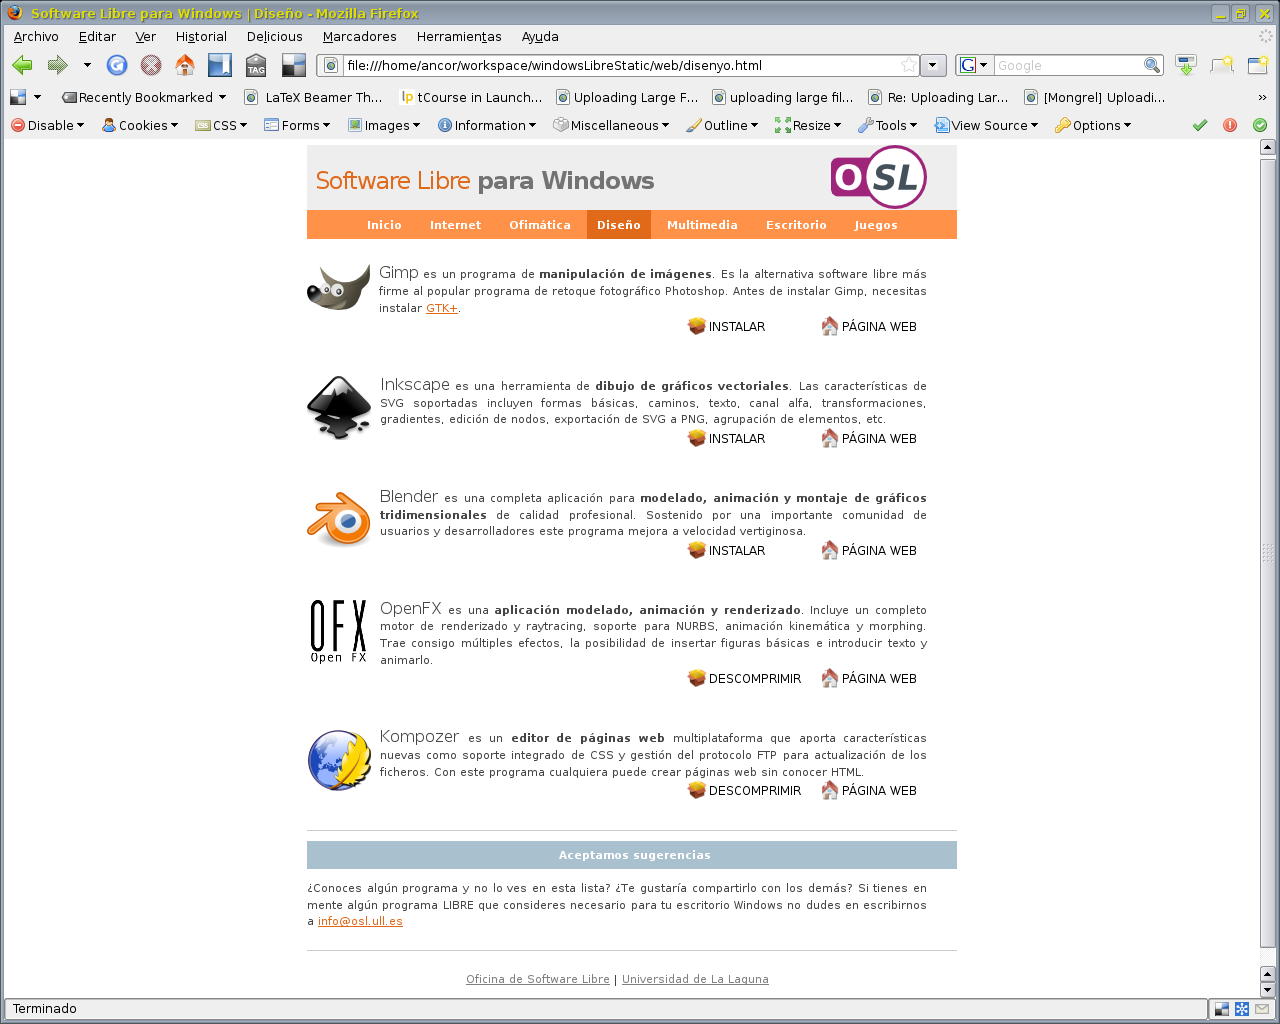
\includegraphics[width=2cm]{images/wl_old02.png}
		\end{columns}
	\end{frame}

	\subsection{¿Que tenemos?} %en alfa1 y que no tenemos
	\begin{frame}
		\frametitle{Windows Libre ALFA 1}
		\setbeamercovered{invisible}
		\begin{itemize}
			\item <1-| alert@1> Una aplicación web dinámica
			\item <2-| alert@2> ''Facilmente mantenible''
			\item <3-| alert@3> Facilidad de incluir nuevas funcionalidades
			\item <4-| alert@4> Ofrecer facilmente contenido extra a cada aplicación
			\item <5-| alert@5> Mayor atractivo visual
			\item <6-| alert@6> Mayor facilidad de uso
			\item <7-| alert@7> Folletos divulgativos
			\item <8-| alert@8> Los CDs se agotaron
			\item <9-| alert@9> ¡Aún queda mucho por hacer!
		\end{itemize}
		% en la columna de la izquierda poner dos capturas de la nueva web
	\end{frame}

	\subsection{¿Que nos depara el futuro?} %en los proximos lanzamientos y en la definitiva (un poquito de fantasia)
	\begin{frame}
		\frametitle{Una aplicación web dinámica}
		\setbeamercovered{invisible}
		\begin{itemize}
			\item <1-| alert@1> Máxima interacción con el usuario
			\item <1-| alert@1> Información aún más accesible %mediante tops, buscador semantico y categorización mediante tags
			\item <1-| alert@1> Más información de cada aplicación
			\item <1-| alert@1> Fidelización de usuarios
			\item <1-| alert@1> Nuevos CDs y DVDs con contenido de interes general
			\item <1-| alert@1> Generación de images CD y DVD con contenido personalizado para descargar
			\item <1-| alert@1> ¿Mac Libre?
		\end{itemize}
	\end{frame}